\chapter{Estruturas Planares de Transmissão}

Muitos meios podem ser utilizados para a realização da transmissão de sinais, tais como: cabos coaxiais, fibras ópticas, o ar entre outros, que dependo da aplicação em que se está trabalhando,	um desses meios será o mais adequado. Cabos coaxiais, por exemplo, são muito utilizados para a criação de redes telefônicas. Entretanto, devido às suas características físicas seu uso acaba limitado para algumas aplicações, como por exemplo, quando há a necessidades de transmissão de um alto volume de dados. As fibras ópticas possibilitam uma alta velocidade de transmissão, ou seja, possibilitam a transmissão de um alto volume de dados em um curto espaço de tempo, e é muito utilizada para transmissões de longas e médias distâncias, porém, para médias distâncias a utilização desse tipo de transmissão necessita de um estudo prévio para analisar a viabilidade de sua utilização, uma vez que os custos envolvendo essa tecnologia são mais elevados do que o de cabos coaxiais, por exemplo. O ar por sua vez é utilizado em aplicações que necessitam da transmissão de informações sem  a utilização de cabos, tecnologia conhecida como \textit{wireless}. Atualmente essa forma de propagação já é muito utilizada; exemplos clássicos que podem ser citados são: rádio difusão, redes de telefonia móvel, redes \textit{wi-fi}, \textit{bluetooth}, entre outras.

Tecnologias que dependem da transmissão via ar fazem uso do espectro eletromagnético e cada tecnologia tem um padrão adotado que utiliza determinada faixa do espectro. Os sinais de rádio e televisão utilizam faixas que vão até 900MHz, os padrões de redes \textit{Wi-Fi IEEE} 802.11(b/n/g) utilizam as faixas 2,3 - 2,4 GHz e 4,9 - 5,9GHz, por exemplo. Para cada tipo faixa de espectro uma tecnologia é adotada para a realização da transmissão de sinais, e no caso das micro-ondas as linhas de transmissões planares são as mais utilizadas.

As estruturas planares de transmissão fazem referências às linhas de transmissão que consistem em tiras condutoras que são impressas na superfície dos substratos das linhas de transmissão. Essas estruturas são a base para circuitos integrados de micro-ondas (MICs), e representam um tópico de pesquisa importante e interessante para muitos engenheiros de micro-ondas. Junto com os avanços em MICs e linhas planares de transmissão, muitos métodos analíticos pra estruturas passivas de micro-ondas e ondas milimétricas, em geral, e linhas planares de transmissão em específico, tem sido desenvolvidos pela necessidade de análise e design mais precisos para os dispositivos MICs. Esses métodos analíticos  têm ajudados na investigação de desenvolvimento de novas linas de transmissão planares.
[\cite{Nguyen}]

A tecnologia planar possibilitou a construção de outras estruturas, como: antenas, ballons, filtros, acopladores ou utilizadas simplesmente para o transporte de sinais. Entre as linhas de transmissão, circuitos impressos, um exemplo de linhas de transmissão planar, são muito úteis na eletrônica moderna. Existem diversos tipos de linhas de transmissão planares, como: \textit{coplanar waveguides} (CPW), \textit{coplanar strip} (CPS), \textit{strip lines}, \textit{slot lines} e a \textit{microstrip}. Dentre todos os tipos de estruturas planares, a \textit{microstrip} é a mais conhecida e comumente usada linha de transmissão planar e foi desenvolvida pelo \textit{ITT Federal Telecommunications Laboratories} em Nutley - Nova Jersey, e publicada por Greig e Engelmann em 1952 [\cite{Grieg}].

\section{Tipos de Estruturas Planares}
Como já mencionado, várias são as formas de linhas de transmissões planares, onde cada tipo de estrutura possui características distintas. Tais características são levadas em consideração na hora das escolha de qual tipo será utilizada para cada tipo de aplicação. Entre as essas características estão a frequência de operação, o espaço necessário para a estrutura, o custo de produção, a facilidade de fabricação, entre outros pontos que precisão ser analisados na escolha. A tabla \ref{tab:propriedades}, lista alguns tipos de estruturas planares com algumas dessas características.

%	Como mencionado anteriormente, existem vários tipos de estruturas planares e cada uma delas tem vantagens e desvantagens, que irão levar a escolha de uma delas para cada um determinado tipo de aplicação. A tabela \ref{tab:propriedades} mostra algumas características de algumas dessas estruturas.

\begin{table}[h]
\begin{center}
\caption{Propriedades de linhas planares de transmissão [\cite{Nguyen}}
\label{tab:propriedades}
	\begin{tabular}{|c c c c c|}
		\hline
		Tipos 				& Frequência de Operação	& Dimensão 	& Perda	& Baixo Custo de Produção \\
		\hline
		Microstrip 			& $\leq$ 110 GHz			& Pequeno	& Alta	& Bom\\
		Strip line 			& $\leq$ 60 GHz				& Médio		& baixa	& Bom\\
		Slot line			& $\leq$ 110 GHz			& Pequena	& Alta	& Bom\\
		Coplanar waveguides & $\leq$ 110 GHz			& Pequeno	& Alta 	& Bom\\
		\hline
	\end{tabular}
	\end{center}
\end{table}

	A seguir são explorados alguns modelos de estruturas planares abordando algumas de suas características e em que aplicações cada tipo de estrutura é utilizada, dando enfase maior para a \textit{microstrip} que é o foco principal da pesquisa.

\subsection{Coplanar Waveguides (CPW)}
	
	\textit{Coplanar waveguides} são um tipo de linha de transmissão planar utilizadas em MICs assim como em \textit{monolitic} MICs (MMICs). A característica principal dessas linhas de transmissão é sua construção uniplanar, ou seja, todos os condutores estão no mesmo lado do substrato. Essa característica facilita a fabricação e permite uma caracterização rápida e econômica utilizando técnicas em wafer.
	
	A CPW foi proposta por C. P. Wen em 1969 que consistia de um substrato dielétrico com condutores na superfície. Os condutores formam uma tira separada por uma pequeno espaço entre dois planos de terra, um de cada lado . As dimensões da tira, do espaçamento entre os planos de terra, a espessura e a permissividade do substrato dielétrico determinam a constante dielétrica efetiva ($\varepsilon_{eff}$), a impedância característica ($Z_0$) e a atenuação ($\alpha$) da linha. Essa estruturas básica passou a ser conhecida como CPW convencional (figura \ref{fig:CPW}) [\cite{Rainee}]

\begin{figure}[htb!]
	\begin{center}
		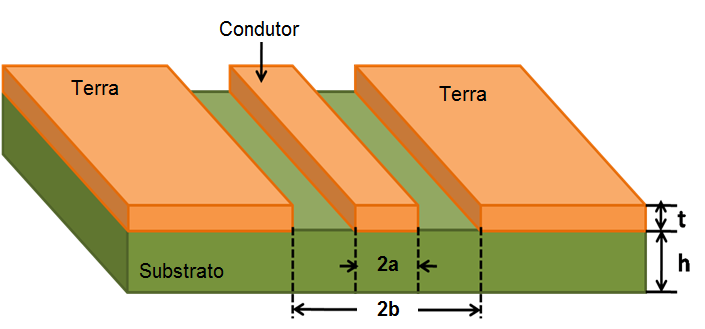
\includegraphics[scale=.5]{./cap1/figuras/coplanar_waveguide.png}
		\caption{Coplanar waveguide}
		\label{fig:CPW}
	\end{center}
\end{figure}
	
Além da estrutura convencional também existem outras formas de CPW que possuem características um pouco diferentes. Entre elas está o \textit{conductor-backed} CPW, ilustrado na figura \ref{fig:backed-CPW}.

\begin{figure}[htb!]
	\begin{center}
		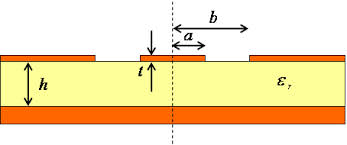
\includegraphics[scale=.6]{./cap1/figuras/backed-CPW.jpg}
		\caption{Conductor-backed coplanar waveguide}
		\label{fig:backed-CPW}
	\end{center}
\end{figure}

As fórmulas utilizadas hoje para a aquisição dos valores de $\varepsilon_{eff}$ e $Z_0$ das estruturas foram derivadas através de métodos de mapeamento conforme (\textit{conformal-mapping}), levando em consideração linhas com espessura zero, e são mostradas a seguir.

Para estruturas coplanares convencionais, segundo \citep{Ghione} temos que:
\begin{equation}
\varepsilon_{eff} = 1+ \frac{\varepsilon - 1}{2}\frac{K(k')}{K(k)}\frac{K(k_1)}{K(k'_1)}
\end{equation}
e 
\begin{equation}
Z_0 = \frac{30\pi}{\sqrt{\varepsilon_{eff}}}\frac{K(k')}{K(k)} 
\end{equation}
onde
\begin{eqnarray}
k &=& \frac{a}{b} \\
k' &=& \sqrt{1-k^2}\\
k_1 &=& \frac{sinh(\pi a/2h)}{sinh(\pi b/2h)}\\
k'_1 &=& \sqrt{1 - k^2_1}
\end{eqnarray}
onde $K(k)$ é a integral elíptica completa de primeira ordem, e seus valores podem ser determinados através da integral ou de através de tabelas.

Devido a importância da integral elíptica de primeira ordem para a análise de vários tipos de linhas de transmissões planares, as equações aproximadas a seguir podem ser utilizadas para o cálculo. [\cite{Hoffmann}]

Para $0 \leq k \leq 0.71$ temos:

\begin{equation}
\label{eq:eliptcal1}
\displaystyle
K(k) = \frac{\pi}{2}\left\lbrace 1+ \frac{2k^2}{8} + \frac{9k^2}{8^2} + 50\left(\frac{k^2}{8}\right)^2 + 306.250\left(\frac{k^2}{8}\right)^4 + ...\right\rbrace
\end{equation}
e para $0.71 <  k \leq 1$
\begin{equation}
\label{eq:eliptcal2}
K(k) = p + \left\lbrace p - 1\right\rbrace\left(\frac{k'^2}{4}\right) + 9\left\lbrace p - \frac{7}{6}\right\rbrace \left(\frac{k'^4}{64}\right) + 25\left\lbrace p - \frac{37}{30}\right\rbrace \left(\frac{k'^6}{256} \right)+ ...
\end{equation}
\begin{equation}
\label{eq:eliptcal3}
p = ln(\frac{4}{k'}) = ln(\frac{4}{\sqrt{1-k^2}})
\end{equation}

O máximo erro relativo das equações \ref{eq:eliptcal1} e \ref{eq:eliptcal2} ocorre o ponto limite $k = \sqrt{0.5} \simeq 0.71$ e é de 3\%. Para $k \rightarrow 0 $ ou $k \rightarrow 1$, o erro relativo em \ref{eq:eliptcal1}, \ref{eq:eliptcal2} e \ref{eq:eliptcal3}, respectivamente, vão para zero. 

Equações simples para a relação $ K(k')/K(k) $ usam projeção estereográfica, definidas por Hilberg, e, para $ 0< k \leq 0.173 $ ou $2 \leq K(k')/K(k) < \infty $, temos as seguintes equações[\cite{Hoffmann}].

\begin{equation}
\label{eq:eliptcal4}
\frac{K(k')}{K(k)} = \left(\frac{4}{\pi} \right) ln\left(\frac{2}{\sqrt{k}}\right)
\end{equation}
\begin{equation}
k = 4 exp\left\lbrace -\frac{\pi K(k')}{2K(k)}\right\rbrace
\end{equation}
e para $ 0.173 < k \leq 1 $ ou $0 \leq K(k')/K(k) < 2 $, temos:
\begin{equation}
\label{eq:eliptcal5}
\frac{K(k')}{K(k)} = \frac{\pi}{ln(2) + 2arctan(\sqrt{k}}
\end{equation}
\begin{equation}
k = \left[tanh\left\lbrace \frac{\pi K(k)}{2K(k') - \frac{ln(2)}{2}}\right\rbrace \right]^2
\end{equation}

O erro relativo para as equações \ref{eq:eliptcal4} e \ref{eq:eliptcal5} é menor que 0.24\%. A função $ K(k')/K(k)$ tende a um valor infinito quando $k=0$, e cai monotonicamente com $k$, chegando a zero quando $k=1$.

A definição completa das integrais elípticas de primeira ordem podem ser encontradas em [\cite{Alan}] e [\cite{Byrd}], Assim como, os resultados também podem ser encontrados já tabelados, como em [\cite{Eugene}]

Quando é levado em consideração a espessura dos condutores, a constante dielétrica efetiva e a impedância característica pode ser calculada da seguinte forma:

\begin{equation}
\displaystyle
\varepsilon_{eff}(t) = \varepsilon_{eff} - \frac{0.7(\varepsilon_{eff}-1)\frac{t}{b-a}}{\frac{K(k)}{K(k')} + 0.7\frac{t}{b-a}}
\end{equation}
e
\begin{equation}
\displaystyle
Z_0 = \frac{30\pi}{\sqrt{\varepsilon_{eff}(t)}}\frac{K(k'_e)}{K(k_e)} 
\end{equation}
onde 
\begin{eqnarray}
\displaystyle
k_e &=& \frac{S_e}{S_e+2W_e}\\
k'_e &=& \sqrt{1 - k^2_e}\\
S_e &=& 2a + \Delta\\
W_e &=& b-a-\Delta\\
\Delta &=&  \frac{1.25t}{\pi} \left[1+\left(\frac{8\pi a}{t}\right)\right]
\end{eqnarray}


\subsection{Microstrip}

Microstrip é uma das formas de estruturas planares mais conhecidas e que é utilizada em diversas aplicações, como antenas e linhas de transmissão dispositivos que trabalhem com RF, principalmente na faixa de ondas milimétricas. Dentre as aplicações de RF mais comuns são as antenas patch, e isso é devido as algumas características que essas estruturas planares possuem, das quais podemos destacar as seguintes:
 \begin{itemize}
 \item Pequena área de ocupação;
 \item Estrutura leve;
 \item Facilidade de fabricação;
 \item Facilidade de  alimentação;
 \item Facilidade para usar em estruturas de array ou em acoplar a outros circuitos microstrip;
 \item Pode assumir qualquer tipo de formato.
 \item Suporta mais de uma frequência de operação.
 \end{itemize}
 
 Porém nem sempre todas as características desse tipo de antenas são vantagens, existem alguns pontos que devem se levados em consideração, como por exemplo a largura de de banda que essas estruturas alcançam, mas que podem ser aumentadas com a utilização de algumas técnicas, ou, por exemplo, quando há a necessidade de isolação do circuito, nesse caso a proteção externa precisa ser considerada.

\begin{figure}[htb!]
	\begin{center}
		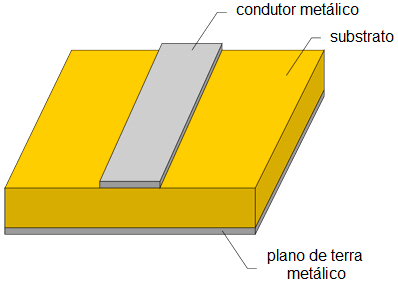
\includegraphics[scale=1]{./cap1/figuras/microstrip.png}
		\caption{Microstrip}
		\label{fig:microstrip}
	\end{center}
\end{figure}

As estrutruas microstrip são  linhas de transmissão geométricas por uma linha condutora simples um dos lados de um substrato dielétrico e um plano de terra simples no lado oposto, como mostrado na figura \ref{fig:microstrip}. Como se trata de uma estrutura aberta, as linhas microstrip tem uma grande vantagem na fabricação comparada com outras estruturas, assim como facilidades para ajustes e interconexões [\cite{Leo}]
%A estruturas microstrip são compostas de uma tira condutora que possui uma largura \emph{w} e espessura \emph{t} e um plano de terra que são separadas por uma camada de material dielétrico (subtrato) de espessura \emph{h} (figura \ref{fig:microstrip}).


A formulas para o cálculo da constante dielétrica efetiva e da impedância característica, hoje já são bem consolidadas, e são mostradas a seguir [\cite{Bhartia}]

\begin{equation}
\varepsilon_{eff} = \frac{\varepsilon_r +1}{2} + \frac{\varepsilon_r -1}{2}\left(1 + \frac{10h}{w}\right)^{-1/2}
\end{equation}
e
\begin{equation}
Z_0 = \frac{42.4}{\sqrt{\varepsilon_r + 1}} ln\left\lbrace 1 + \frac{4h}{w} \left[  G + \sqrt{ G^2 + \frac{\pi^2}{2} \left(  1 + \frac{1}{\varepsilon_r}\right)}\right] \right\rbrace
\end{equation}
onde
\begin{equation}
G =  \left(\frac{14 + \frac{8}{\varepsilon_r}}{11}\right)\frac{4h}{w} 
\end{equation}

\section{Aplicações de Estruturas Planares}

Como já mencionado, as linas de transmissões planares podem ser utilizadas em diversas aplicações devido a suas características físicas, principalmente facilidade de fabricação e integração com outros dispositivos, dentre elas as antenas de micro fita são as mais comuns e são utilizadas nas mais diversas formas de comunicações, em [\cite{Patel}] é foi feito um levantamento de alguns tipos de comunicação que utilização antenas de micro fita, entre elas estão: comunicações móveis, GPS, identificação em radiofrequência (RFID), radar e WiMAx. Mas além de antenas de microfita as estruturas planares também podem ser utilizadas para fabricação de outros dispositivos como anéis de ressonância [\cite{Benjamin}], superfícies seletoras de frequências [\cite{Mauricio}], entre outras.

%Como já mencionado, as linhas planares de transmissão, são muito úteis para algumas aplicações devido as suas características físicas, principalmente pela facilidade de fabricação de tais estruturas. Mas onde tais estruturas podem ser aplicadas para solucionar determinados problemas? Em mutias áreas voltadas para a criação de sistemas, utilizam de alguma forma linhas de transmissões planares, umas das áreas onde mais há esforços a fim de desenvolver tais estruturas é a área de RF, mas especificamente, micro-ondas.

\section{Resumo do Capítulo}

Neste Capítulo buscou mostrar algumas formas de estruturas de transmissões planares que podem ser encontradas hoje, assim como fornecer uma base teórica mínima de como uma estrutura planar pode ser projetada, levando em consideração suas dimensões físicas, como largura da linha de transmissão e a espessura dos dielétricos, assim como mostrar algumas aplicações onde tais estruturas são comumente utilizadas.